\documentclass[12pt]{report}
\usepackage{graphicx}
\usepackage{array}
\usepackage{tabularx}
\usepackage{amsmath}
\usepackage{hyperref}
\usepackage{geometry}
\usepackage{fontspec} % For custom fonts
\usepackage{xcolor}
\usepackage{float}
\usepackage{titling}
\usepackage{tikz}
\usepackage{fancyhdr} % For custom headers/footers
\usepackage{tocbibind} % To include TOC, LOF, LOT in TOC
\setmainfont{Times New Roman} % Set the main font to Times New Roman
\geometry{a4paper, margin=1in}
\usepackage{setspace}
\onehalfspacing 
\usepackage{titlesec}
\usepackage{fancyhdr}
\usepackage[titles]{tocloft}
\usepackage{chngcntr}

\counterwithout{figure}{chapter}
\counterwithout{table}{chapter}

\renewcommand{\tablename}{Tableau}
\renewcommand{\cftpartpresnum}{PARTIE~} 
\renewcommand{\cftpartaftersnum}{.}     
\renewcommand{\cftpartleader}{\cftdotfill{\cftdotsep}}
\setlength{\cftpartnumwidth}{5em}

\renewcommand{\cftchappresnum}{Chapitre~}
\renewcommand{\cftchapaftersnum}{.}     
\renewcommand{\cftchapleader}{\cftdotfill{\cftdotsep}}
\setlength{\cftchapnumwidth}{5em}

\pagestyle{fancy}
\fancyhf{} % Clear all header and footer fields
\fancyfoot[C]{\thepage} % Place the page number in the center of the footer
\renewcommand{\headrulewidth}{0pt}  % Removes the line in the header
\renewcommand{\footrulewidth}{0pt}  % Removes the line in the footer
\hypersetup{
   colorlinks=true,
  linkcolor=black,   % Set link color to black
  filecolor=magenta, 
  urlcolor=cyan,
  pdfborder={0 0 0} 
}
\renewcommand{\contentsname}{SOMMAIRE GENERAL} 
\renewcommand{\listtablename}{LISTE DES TABLEAUX}
\renewcommand{\listfigurename}{LISTE DES FIGURES}
\newcommand{\figref}[1]{figure \ref{#1}}

\titleformat{\part}[display]
  {\normalfont\Huge\bfseries\centering}
  {PARTIE \Roman{part}}{20pt}{\Huge}

\titleformat{\chapter}[display]
  {\normalfont\Large\bfseries\centering}
  {Chapitre \arabic{chapter}~.}{20pt}{\Large}

\titleformat{\section}
    {\normalfont\large\bfseries} 
    {\thesection}
    {1em}
    {\large}
	
\begin{document}	
			 \pretitle{
				\begin{tikzpicture}[remember picture, overlay]
			   		\node[anchor=north west, xshift=1.5cm, yshift=-1cm] at (current page.north west) {
        						\includegraphics[width=2.5cm]{image1.png}
					};
    					\node[anchor=north west, xshift=4cm, yshift=-1cm] at (current page.north west) {
        						\includegraphics[width=2.3cm]{image2.png}
					};
					\node[anchor=north east, xshift=-1.5cm, yshift=-1cm] at (current page.north east) {
        						
\includegraphics[width=5cm]{image3.png}
					};
				\end{tikzpicture}
				\begin{center}
					\textbf{\large UNIVERSITE DE FIANARANTSOA ECOLE NATIONALE D'INFORMATIQUE \\[0.5cm] MEMOIRE DE FIN D'ETUDES POUR L'OBTENTION DU DIPLOME DE MASTER PROFESSIONNELLE}
					\\[0.5cm]
							\textbf{\underline{Mention:}} Informatique \\	
							\textbf{\underline{Parcours:}} Informatique générale\\
							\textbf{\textit{Intitulé}}				\end{center}
				\begin{center}\Large\bfseries
			}
			\preauthor{\begin{flushleft}\fontsize{12} \lineskip Présenté le 01 février 2023 }
			\postauthor{\end{flushleft} \textbf{Membres du Jury:} 
			 \begin{itemize}
			    \item \textbf{Président:} Monsieur RALAIVAO Jean Christian, Assistant d'Enseignement Supérieur et de Recherche;
			    \item \textbf{Examinateur:} Monsieur RALAIVAO Jean Christian, Assistant d'Enseignement Supérieur et de Recherche;
			    \item \textbf{Rapporteurs:} \begin{itemize}
       									 \item Monsieur RALAIVAO Jean Christian, Assistant d'Enseignement Supérieur et de Recherche;
       									 \item Monsieur RALAIVAO Jean Christian, Assistant d'Enseignement Supérieur et de Recherche.
    								\end{itemize}
			\end{itemize} }
			\predate{\begin{flushright} Année Universitaire: }
			\postdate{\end{flushright}}
			\title{
				\color{blue}
				\setlength{\fboxsep}{10pt} 
				\begin{center}
					\fbox{
						\begin{minipage}{0.95\textwidth}
							\begin{center}
								CONCEPTION ET REALISATION  D'UNE APPLICATION WEB  DE RESERVATION DE VOYAGE
							\end{center}
						  \end{minipage}
					}
				\end{center}
			}
			\author{\textbf{Par:} Monsieur ANDRIAMIORA Ainamalala Lucky}
			\date{2024-2025}
			\maketitle
			
			\newpage
			\thispagestyle{empty}
			\mbox{}

			\newpage
			\pagenumbering{roman}
			\renewcommand{\thepage}{\Roman{page}} % Ensure uppercase Roman numerals
			\setcounter{page}{1}
			\chapter*{CURRICULUM VITAE}
			\addcontentsline{toc}{chapter}{CURRICULUM VITAE}	
			\begin{center}
				\begin{minipage}{0.6\textwidth}
					\textbf{Nom:} ANDRIAMIORA\\
					\textbf{Prenom:} Ainamalala Lucky\\
					\textbf{Numéro:} +261 34 33 513 61\\
					\textbf{Addresse:} IIG20 E Ambatomaro, Antananarivo\\
					\textbf{E-mail:} luckyainamalalalucky@gmail.com\\
					\textbf{Date et lieu de naissance:} 30 décembre 1999 à Antsirabe
				\end{minipage}
				\hfill
				\begin{minipage}{0.3\textwidth}
					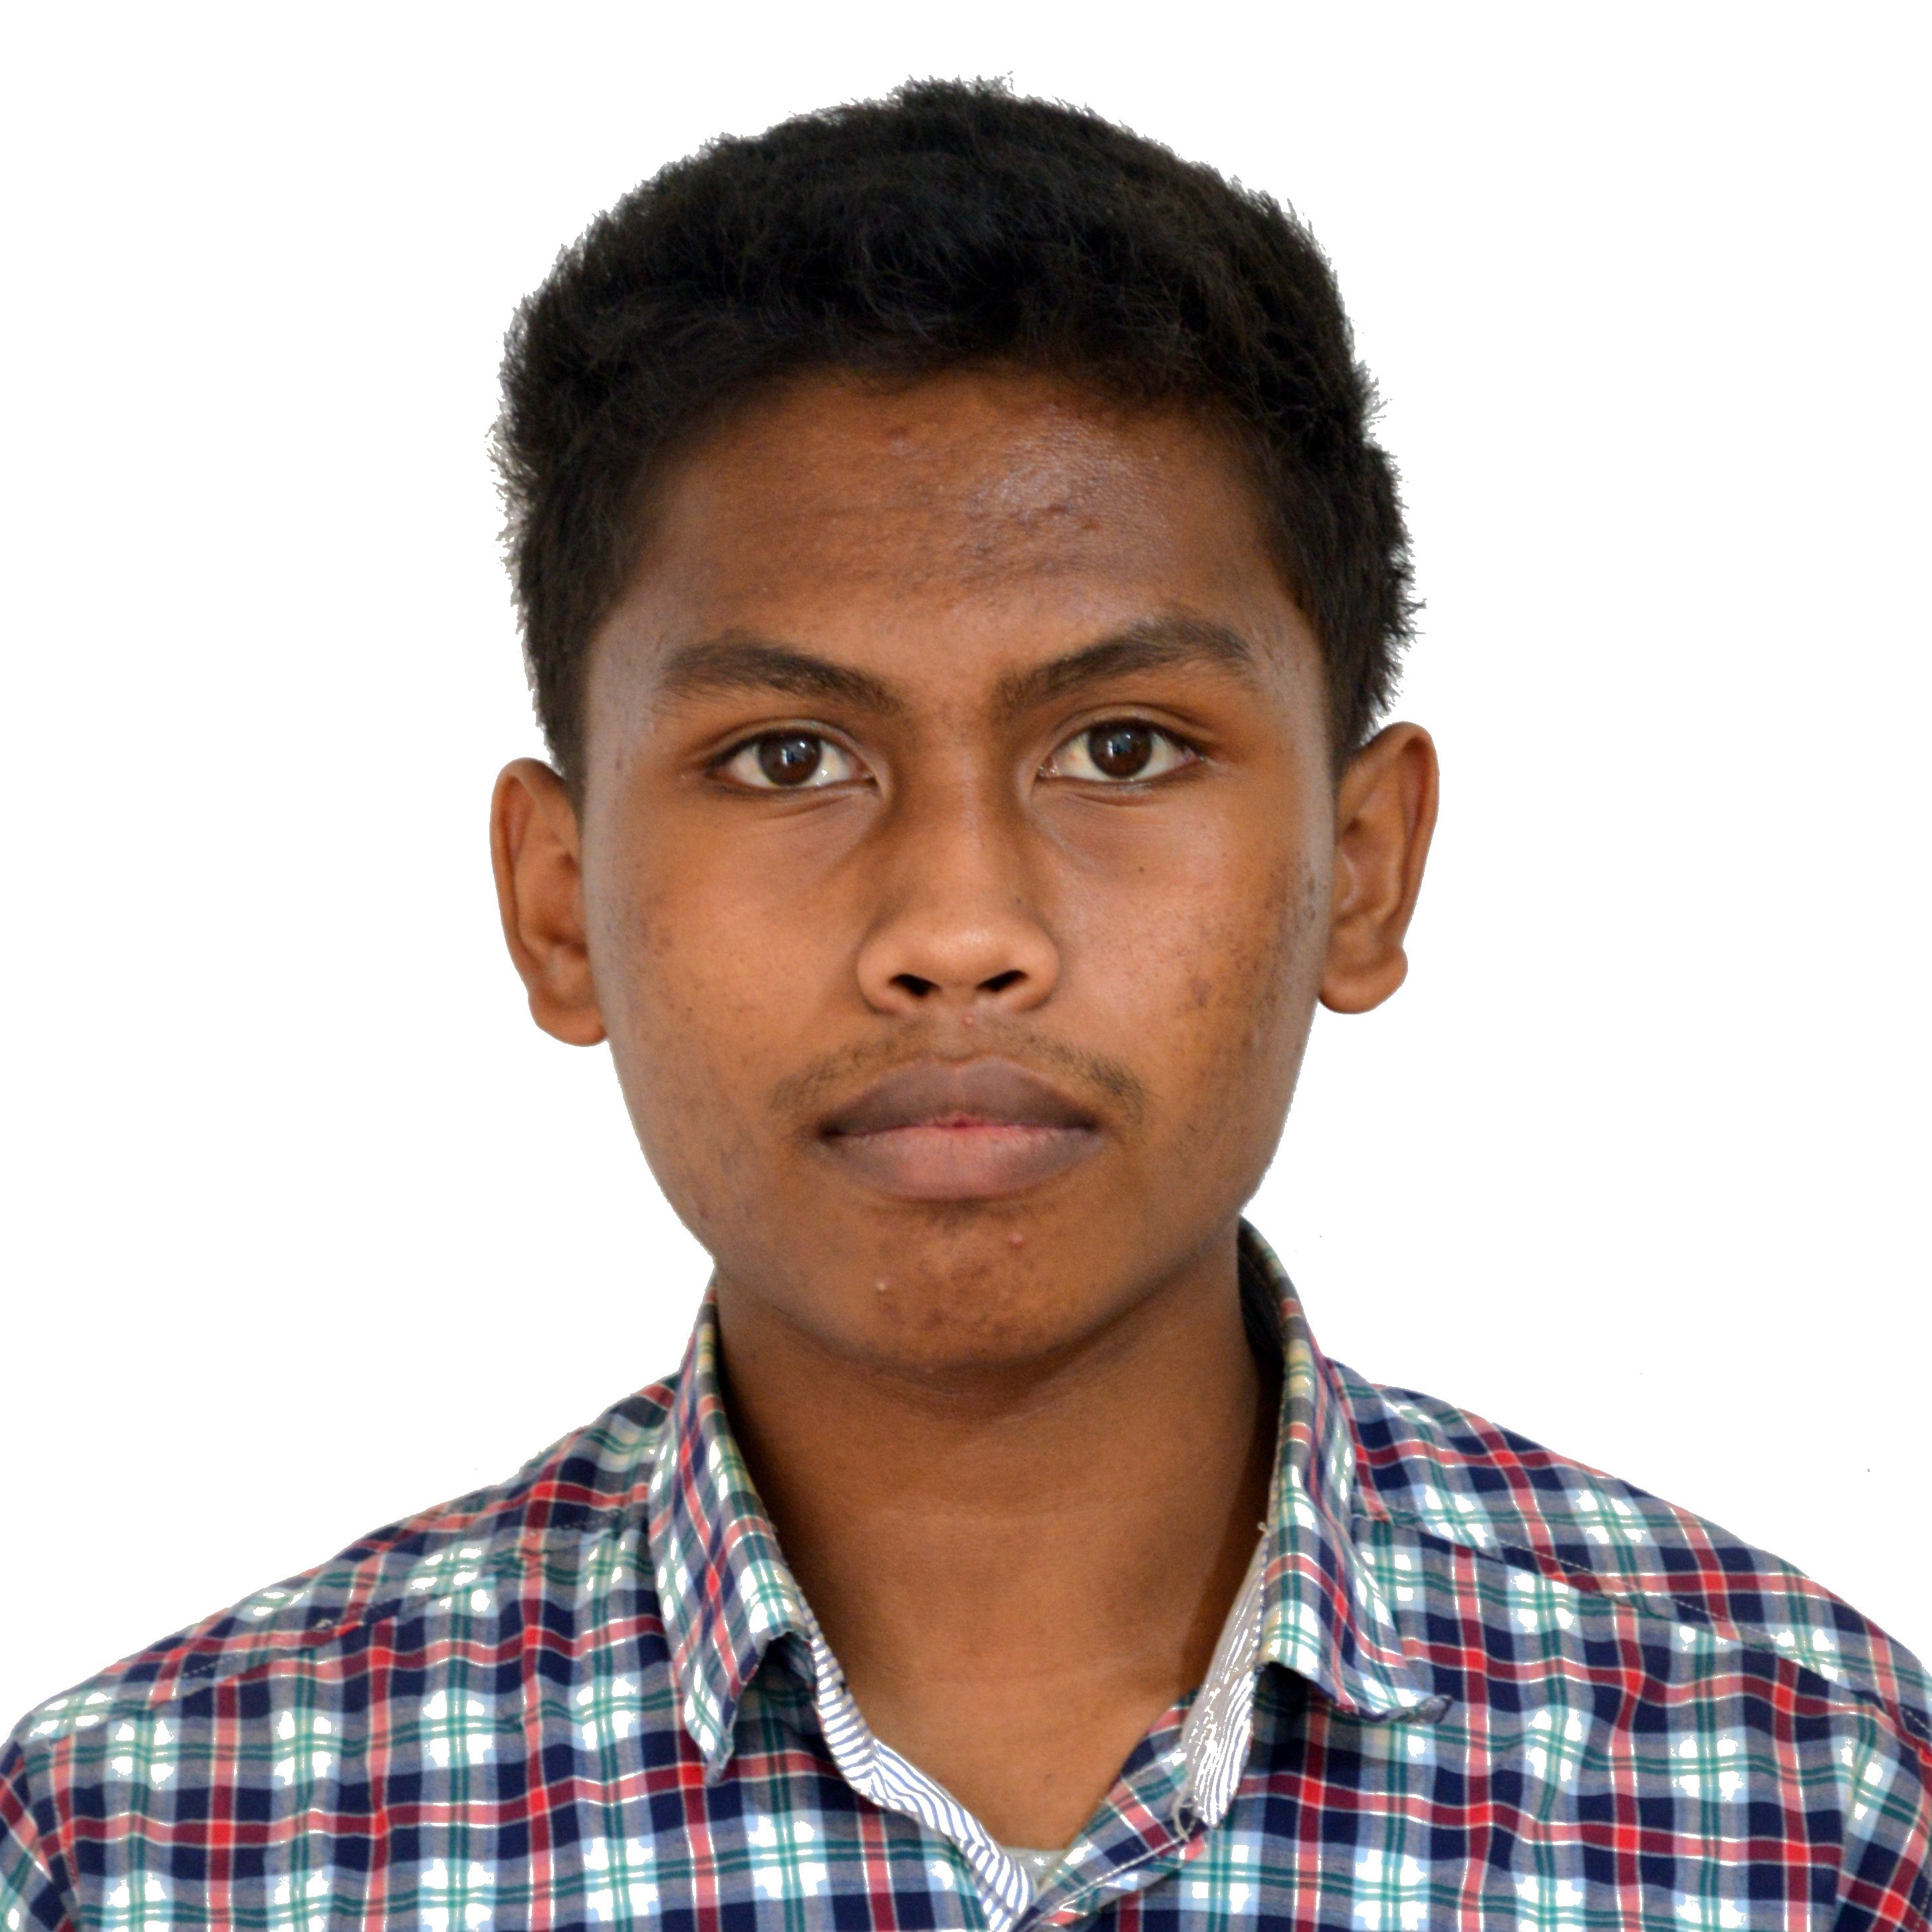
\includegraphics[width=3.5cm, height=3.5cm]{mypic.jpg}	
				\end{minipage}
			\end{center}
			\section*{FORMATIONS ET DIPLOME}
			\begin{center}
				\begin{minipage}{\textwidth}
					\textbf{2024-2025:} Deuxième année de formation en Master professionnelle à l’École Nationale d'Informatique, Université de Fianarantsoa, parcours : Informatique générale.\\[0.5cm]
					\textbf{2023-2024:} Première année de formation en Master professionnelle à l’École Nationale d'Informatique, Université de Fianarantsoa, parcours : Informatique générale.\\[0.5cm]
					\textbf{2022-2023:} Obtention du diplôme de Licence professionnelle mention Bien à l’École Nationale d'Informatique, Université de Fianarantsoa, parcours : Informatique générale.\\[0.5cm]
					\textbf{2021-2022:} Deuxième année de formation en Licence professionnelle à l’École Nationale d'Informatique, Université de Fianarantsoa, parcours : Informatique générale.\\[0.5cm]
					\textbf{2020-2021:} Première année de formation en Licence professionnelle à l’École Nationale d'Informatique, Université de Fianarantsoa, parcours : Informatique générale.\\[0.5cm]
					\textbf{2019-2020:} Obtention du diplôme de Baccalauréat série D mention assez-bien au Lycée André Résampa Antsirabe.
				\end{minipage}
			\end{center}
			\section*{STAGES ET EXPERIENCES PROFESSIONNELLES}
			\begin{center}
				\begin{minipage}{\textwidth}
       					 \textbf{11 juin 2024 au 4 novembre 2024:} Stage auprès de Nexitia technologies.
						\begin{itemize}
							\item Thème du stage: Application web Handeha voyage;
							\item Langages et outils: Java, spring boot, JavaScript, next js, Katappult, H2, UML.						
						\end{itemize}
       					 \textbf{Octobre 2023:} Projet à l’École Nationale d'Informatique.
						\begin{itemize}
							\item Thème du stage: Module de securité pour application spring boot et angular;
							\item Langages et outils: Java, spring boot, Angular, TypeScript, PostgreSQL, UML.						
						\end{itemize}       					 
					\textbf{19 octobre 2022 au 16 janvier 2023:} Stage auprès de la Paositra malagasy.
						\begin{itemize}
							\item Thème du stage: Application web pour la gestion des change;
							\item Langages et outils: Java, spring boot, Angular, TypeScript, PostgreSQL, UML.								
						\end{itemize}
					\textbf{Septembre 2022:} Projet à l’École Nationale d'Informatique.
						\begin{itemize}
							\item Thème du stage: Création d'une application mobile de gestion de cotisation de groupe;
							\item Langages et outils: Java, Android Studio.								
						\end{itemize}
					\textbf{8 mars 2021 au 7 juillet 2021:} Stage auprès du Ministère de l’Économie et de la Finance.
						\begin{itemize}
							\item Thème du stage: Application web pour la gestion des dossier du personnels de la Direction du Système d'Information;
							\item Langages et outils: Java, spring boot, Angular, TypeScript, PostgreSQL, UML.								
						\end{itemize} 
					\textbf{Avril 2021:} Projet à l’École Nationale d'Informatique.
						\begin{itemize}
							\item Thème du stage: Réalisation d’une application desktop de Gestion des heures complémentaires;
							\item Langages et outils: Php, MySQL, Ajax.								
						\end{itemize} 
					\textbf{Août 2020:} Projet à l’École Nationale d'Informatique.
						\begin{itemize}
							\item Thème du stage: Création d'une application desktop de gestion de stock;
							\item Langages et outils: C++, Qt Creator.								
						\end{itemize} 
   				\end{minipage}		
			\end{center}
			\section*{CONNAISSANCES EN INFORMATIQUE}
			\begin{center}
				\begin{minipage}{\textwidth}
					\begin{itemize}
						\item \textbf{Systèmes d'exploitation:} Microsoft Windows, Linux;
						\item \textbf{Langages de Programmation:} Java, JavaScript, TypeScript, Python , C/C++;
						\item \textbf{Développement Web:} HTML5, CSS3, Tailwind CSS, React.js, Next.js, Angular, Node.js, Express.js;
						\item \textbf{Développement Backend:} Spring Framework, Node.js, Express.js;
						\item \textbf{Compétences en bases de données:} SQL, PostgreSQL, MySQL;
						\item \textbf{Outils de Gestion de Versions:} Git, GitHub, GitLab; 	
						\item \textbf{Outils DevOps:} Docker, Kubernetes, Jenkins, Ansible;
						\item \textbf{Outils de virtualisation:} Docker, VirtualBox, VMware, Vagrant; 	
						\item \textbf{Outils de tests et Assurance Qualité:} Jest, JUnit;
						\item \textbf{Outils et Méthodologies de Conception et Gestion de Projets Logiciels:} UML, Méthodologie Agile, 2TUP, MERISE, GRASP;
						\item \textbf{Outils de Documentation et de Préparation de Contenu:} LaTeX/TeX.	
					\end{itemize}
	   			\end{minipage}		
			\end{center}
			\section*{CONNAISSANCES LINGUISTIQUE}
			\begin{center}
				\begin{minipage}{\textwidth}
					\begin{center}
						\begin{tabularx}{\textwidth}{|c|X|X|X|X|}
							\hline
							\textbf{LANGUE} & \textbf{COMPREHENSION} & \textbf{LECTURE} & \textbf{PARLE} & \textbf{ECRIT}\\
							\hline
							Anglais & Bien & Bien & Assez-bien & Bien \\
							\hline
							Français & Bien & Bien & Bien & Bien\\
							\hline
						\end{tabularx}
					\end{center}
				\end{minipage}
			\end{center}
			\section*{LOISIR ET CENTRES D'INTERET}
			\begin{center}
				\begin{minipage}{\textwidth}
					\begin{itemize}
						\item Musique;
						\item Podcast;
						\item Documentaires;
						\item Anime;
						\item Jeux video;
						\item	Lecture.
					\end{itemize}
				\end{minipage}	
			\end{center}
			\chapter*{REMERCIEMENTS}
			\addcontentsline{toc}{chapter}{REMERCIEMENTS}	
			\begin{center}
				\begin{minipage}{\textwidth}
					\hspace{15pt} Avant toute chose, je tiens à remercier Dieu tout puissant et miséricordieux, qui m'a donné la force et la patience d'accomplir ce modeste travail.\\[0.5cm]
					Mes remerciements s’étendent également à :
					\begin{itemize}
						\item Monsieur HAJALALAINA Aimé Richard, Docteur HDR, Président de l'Université de Fianarantsoa, pour tout ce qu'il entreprend à l'Université;
						\item Monsieur MAHATODY Thomas, Docteur HDR, Directeur de l’École Nationale d'Informatique, qui nous à donné l'opportunité d'aller en stage pour ainsi permettre d’accroître nos compétences;
						\item Monsieur RANARISON Richard, Directeur Général de la Paositra Malagasy, pour son accueil et la confiance qu'il à accordée depuis mon arrivée dans l’établissement;
						\item Monsieur RATIARSON Venot, Maître de Conférences, mon encadreur pédagogique, pour ses conseils et échanges tout au long du stage;
						\item Madame RANDRIAMIHARISOA Rollande, mon encadreur professionnelle, qui m'a toujours guidée lors de la réalisation du projet;
						\item Monsieur RALAIVAO Jean Christian, Assistant d'Enseignement Supérieur et de Recherche,d’avoir accepté de présider la soutenance;
					 	\item Monsieur DIMBISOA William Germain, Docteur en Informatique, d'avoir accepté d'examiner mon présent travail;
						\item Toutes les personnels de la Paositra Malagasy, pour leurs accueils;
						\item Toutes les enseignants et les personnels de l’École Nationale d'Informatique qui se sont acharné à nous former durant l'année universitaire;
						\item Ma famille pour son soutien, que se soit moral, matériel ou financier.
					\end{itemize}
				\end{minipage}
			\end{center}
			\newpage
			\tableofcontents
			\newpage
			\chapter*{NOMENCLATURE}
			\addcontentsline{toc}{chapter}{NOMENCLATURE}	
			\newpage
			\listoftables
			\newpage
			\listoffigures
			\newpage
			\newpage
			\pagenumbering{arabic}
			\setcounter{page}{1}
			\chapter*{INTRODUCTION GÉNÉRALE}
			\addcontentsline{toc}{chapter}{INTRODUCTION GÉNÉRALE}
			\begin{center}
				\begin{minipage}{\textwidth}
					\hspace{15pt} Avec sa biodiversité unique et sa richesse culturelle, Madagascar est une destination touristique de choix. Cependant, avec la demande pour des expériences de voyage personnalisées et accessibles en ligne en constante croissance, de nombreux opérateurs touristiques luttent pour obtenir la visibilité et les moyens nécessaires pour promouvoir efficacement leurs offres.\\
	
					\hspace{15pt} Malgré l'essor des plateformes de réservation en ligne, il demeure un besoin urgent d'une solution centralisée pour permettre aux opérateurs touristiques malgaches de partager leurs offres et aux voyageurs de réserver facilement leurs circuits ou séjours.\\
	
					\hspace{15pt} L'objectif de ce mémoire est de développer et de présenter "Handeha Voyage", une application web qui  facilite la mise en ligne des offres de circuits et de séjours par les opérateurs touristiques, simplifie le processus de réservation pour les utilisateurs et améliore la visibilité des opérateurs touristiques. Cette étude propose une solution novatrice qui répond directement aux défis rencontrés par les opérateurs touristiques et les voyageurs à Madagascar. En effet, l'application "Handeha Voyage" ne se contente pas de faciliter la réservation des voyages; elle redéfinit fondamentalement la manière dont les services touristiques sont présentés et consommés.\\
	
					\hspace{15pt} Ce mémoire abordera le processus de conception, de développement et de mise en œuvre de l'application "Handeha Voyage". Nous utiliserons des méthodes de conception et de modélisation adaptées, ainsi que des langages de programmation et frameworks appropriés, sans oublier un système de gestion de base de données solide. Tout cela sera orchestré selon une méthodologie de gestion de projet bien définie pour assurer une organisation optimale. Les limitations incluent le temps limité pour le développement complet de certaines fonctionnalités avancées, l'accès limité aux données et la difficulté à recueillir des retours d'expérience durant le développement.\\
	
					\hspace{15pt} Notre plan se subdivise en trois parties: dans un premier temps la présentation de l’École Nationale d'Informatique (ENI) suivie de celle de Nexitia Technology. Dans la deuxième partie, nous aborderons les analyses et la conception du projet. Enfin, la troisième partie portera sur la réalisation du projet avec les différents moyens et outils utilisés.
				\end{minipage}
			\end{center}
			\part{PRESENTATION}
			\chapter{Présentation de l’Ecole Nationale d’Informatique}
			\section{Information d’ordre générale }
				\hspace{15pt} L’Ecole Nationale d’Informatique, en abrégé ENI, est un établissement d’enseignement supérieur rattaché académiquement et administrativement à l’Université de Fianarantsoa. Le siège de l’Ecole se trouve à Tanambao-Antaninarenina à Fianarantsoa. L’adresse pour la prise de contact avec l’Ecole est la suivante : Ecole Nationale d’Informatique (ENI) Tanambao, Fianarantsoa. Le numéro de sa boîte postale est 1487 avec le code postal 301. Téléphone : 034 05 733 36 ou 032 15 204 28. Son adresse électronique est la suivante : eni@eni.mg. Il dispose également d'un site web : \textbf{www.eni.mg}
			\section{Missions et historiques}
				\hspace{15pt} L’ENI se positionne sur l’échiquier socio-éducatif malgache comme étant le plus puissant secteur de diffusion et de vulgarisation des connaissances et des technologies informatiques. 

				Cette Ecole Supérieure peut être considérée aujourd’hui comme la vitrine et la pépinière des élites informaticiennes du pays.
	
				L’Ecole s’est constituée de façon progressive au sein du Centre Universitaire Régional (CUR) de Fianarantsoa.

				De façon formelle, l’ENI était constituée et créée au sein du (CUR) par le décret N° 83- 185 du 24 Mai 1983, comme étant le seul établissement Universitaire Professionnalisé au niveau national, destiné à former des techniciens et des Ingénieurs de haut niveau, aptes à répondre aux besoins et exigences d’Informatisation des entreprises, des sociétés et des organes implantés à Madagascar.

				           \begin{center}
						\begin{minipage}{\textwidth}
								\hspace{15pt} L’ENI a pour conséquent pour mission de former des spécialistes informaticiens compétents et opérationnels de différents niveaux notamment : 
				
								\begin{itemize}
									\item En fournissant à des étudiants des connaissances de base en informatique ;
									\item En leur transmettant le savoir-faire requis, à travers la professionnalisation des formations dispensées et en essayant une meilleure adéquation des formations par rapport aux besoins évolutifs des sociétés et des entreprises ;
									\item En initiant les étudiants aux activités de recherche dans les différents domaines des Technologies de l’information et de la communication (TIC).\\
								\end{itemize}
						\end{minipage}
					\end{center}

				L’implantation de cette Ecole Supérieure de technologie de pointe dans un pays en développement et dans une Province (ou Faritany) à tissu économique et industriel faiblement développé ne l’a pourtant pas défavorisée, ni empêchée de former des spécialistes informaticiens de bon niveau, qui sont recherchés par les entreprises, les sociétés et les organismes publics et privés sur le marché de l’emploi.

				La filière de formation d’Analystes Programmeurs a été mise en place à l’Ecole en 1983, et a été gelée par la suite en 1996, tandis que la filière de formation d’ingénieurs a été ouverte à l’Ecole en 1986.
				
				Dans le cadre du Programme de renforcement en l’Enseignement Supérieur (PRESUP), la filière de formation des Techniciens Supérieurs en Maintenance des Systèmes des informatiques a été mise en place en 1986 grâce à l’appui matériel et financier de la Mission Française de coopération auprès de l’Ambassade de France à Madagascar.

				Une formation pour l’obtention de la certification CCNA et / ou NETWORK +. Appelée « CISCO Networking Academy » a été créée à l’Ecole en 2002-2003 grâce au partenariat avec CISCO SYSTEM et l’Ecole Supérieure Polytechnique d’Antananarivo (ESPA). Cependant, cette formation n’avait pas duré longtemps. Une formation de troisième cycle a été ouverte à l’Ecole a été ouverte à l’Ecole depuis l’année 2003 – 2004 grâce à la coopération académique et scientifique entre l’Université de Fianarantsoa pour le compte de l’ENI et l’Université Paul Sabatier de Toulouse (UPST).
				
				 \begin{center}
					 \begin{minipage}{\textwidth}
	
						\hspace{15pt} Cette filière avait pour objectif de former certains étudiants à la recherche dans les différents domaines de l’Informatique, et notamment pour préparer la relève des Enseignants-Chercheurs qui étaient en poste. Pendant l’année 2007-2008, la formation en vue de l’obtention du diplôme de Licence Professionnelle en Informatique a été mise en place à l’ENI avec les deux options suivantes de formation :
						
						\begin{itemize}
							\item Génie Logiciel et base de Données.
							\item Administration des Système et réseaux.\\
						\end{itemize}
					\end{minipage}

				\end{center}
				
				La mise en place à l’Ecole de ces deux options de formation devait répondre au besoin de basculement vers le système Licence – Master – Doctorat (LMD). Mais la filière de formation des Techniciens Supérieurs en Maintenance des Systèmes Informatiques a été gelée en 2009. 
En vue de surmonter les difficultés de limitation de l’effectif des étudiants accueillis à l’Ecole, notamment à cause du manque d’infrastructures, un système de « Formation Hybride » a été mise en place à partir de l’année 2010. Il s’agit en effet d’un système de formation semi présentielle et à distance avec l’utilisation de la visioconférence pour la formation à distance. Le système de formation hybride a été ainsi créé à Fianarantsoa ainsi qu’Université de Toliara.

				\section{Organigramme institutionnel}

				\hspace{15pt} Cet organigramme de l’Ecole est inspiré des dispositions du décret N° 83-185 du 23 Mai 1983.

				L’ENI est administrée par un conseil d’Ecole, et dirigée par un directeur nommé par un décret adopté en conseil des Ministres.

				Le Collège des enseignants regroupant tous les enseignants-chercheurs de l’Ecole est chargé de résoudre les problèmes liés à l’organisation pédagogique des enseignements ainsi que à l’élaboration des emplois du temps.

				\begin{center}
					\begin{minipage}{\textwidth}
						\hspace{15pt} Le Conseil Scientifique propose les orientations pédagogiques et scientifiques de l’établissement, en tenant compte notamment de l’évolution du marché de travail et de l’adéquation des formations dispensées par rapport aux besoins des entreprises. Trois départements de formation caractérisent l’organigramme :
						\begin{itemize}
							\item Le département de formation théorique à l’intérieur de l’Ecole ;
							\item Le département de formation pratique pour la coordination et la supervision des stages en entreprise et des voyages d’études ;
							\item Le département de formation doctorale pour l’organisation de la formation de 3ème cycle. La figure \ref{fig:figure 1} présente l’organigramme actuel de l’Ecole.
						\end{itemize}
					\end{minipage}
				\end{center}
				\begin{figure}[h]
					\centering
					\includegraphics[width=\textwidth]{image4.png}
					\caption{Organigramme institutionnel de l'ENI}
					\label{fig:figure 1}
				\end{figure}
				\clearpage
				
				Sur cet organigramme, l’Ecole placée sous la tutelle académique et administrative de l’Université de Fianarantsoa, et dirigée par un Directeur élu par les Enseignants – Chercheurs permanents de l’Etablissement et nommé par un décret pris en Conseil des ministres pour un mandat de 3 ans. 

				Le Conseil de l’Ecole est l’organe délibérant de l’Ecole.

				Le Collège des Enseignants propose et coordonne les programmes d’activités pédagogiques. Le Conseil scientifique coordonne les programmes de recherche à mettre en œuvre à l’Ecole. Le Secrétariat principal coordonne les activités des services administratifs (Scolarité, Comptabilité, et Intendance). Conformément aux textes en vigueur régissant les Etablissements malgaches d’Enseignement Supérieur, qui sont barrés sur le système LMD, les Départements de Formation pédagogique ont été ainsi remplacés par des Mentions et des parcours.

				Et les chefs des Départements ont été ainsi remplacés par des responsables des mentions et les responsables des parcours. Un administrateur des Réseaux et Systèmes gère le système d’information de l’Ecole et celui de l’Université.
	
				\section{Domaine de spécialisation}

				\begin{center}
					\begin{minipage}{\textwidth}
						\hspace{15pt} Les activités de formation et de recherche organisées à l’ENI portent sur les domaines suivants : 
						\begin{itemize}
							\item Génie logiciel et Base de Données ;
							\item Administration des Systèmes et Réseaux ;
							\item Informatique Générale ;
							\item Modélisation informatique et mathématique des Systèmes complexes.\\
						\end{itemize}
					\end{minipage}
				\end{center}
				D’une manière plus générale, les programmes des formations sont basés sur l’informatique de gestion et sur l’informatique des Systèmes et Réseaux. Et les modules de formation intègrent aussi bien des éléments d’Informatique fondamentale que des éléments d’Informatique appliquée. Le tableau \ref{tab:tableau 1} décrit l’organisation du système de formation pédagogique de l’Ecole.

				\begin{table}[h]
				  \centering
				  \caption{Organisation du système de formation pédagogique de l’Ecole}
				  \label{tab:tableau 1}
					  \begin{tabular}{|p{7cm}|p{7cm}|}
					    \hline
					    Formation Théorique & Formation Pratique \\
					    \hline
					    \begin{itemize}
						\item Enseignement théorique
						\item Travaux dirigés
						\item Travaux pratiques
						\item Conférences
					    \end{itemize}
					 &  
					\begin{itemize}
						\item Etude de cas
						\item Travaux de réalisation
						\item Projets/ Projets tutoriels
						\item Voyages d’Etudes
						\item Stages en entreprise
					\end{itemize}
					\\
					    \hline
					  \end{tabular}
				\end{table}
				\clearpage

				\section{Architecture des formations pédagogiques}

				\hspace{15pt} Le recrutement des étudiants à l’ENI se fait uniquement par voie de concours d’envergure nationale en première année.

				Les offres de formation organisées à l’Ecole ont été validées par la Commission Nationale d’Habilitation (CNH) auprès du Ministères de l’Enseignement Supérieur et de la Recherche Scientifique selon les dispositions de l’Arrêté N°31.174/2012-MENS en date du 05 Décembre 2012.

				\begin{center}
					\begin{minipage}{\textwidth}
						\hspace{15pt} Au sein de l’ENI, il existe une seule mention (INFORMATIQUE) et trois parcours :
						\begin{itemize}
							\item Génie logiciel et Base de Données ;
							\item Administration des Systèmes et Réseaux ; 
							\item Informatique Générale.\\
						\end{itemize}
					\end{minipage}	
				\end{center}

				L’architecture des études à trois niveaux conforment au système Licence- Master-Doctorat (LMD) permet les comparaisons et les équivalences académiques des diplômes au niveau international. 

				\begin{itemize}
					\item L = Licence (Bac + 3) = L1, L2, L3 = 6 semestres S1 à S6.

						Le diplôme de licence est obtenu en 3 années des études après Baccalauréat. Et le diplôme de Master est obtenu en 2 ans après obtenu du diplôme de LICENCE. Le MASTER PROFESSIONNEL est un diplôme destiné à la recherche emploi au terme des études.

					\item M = Master (Bac + 5) = M1, M2 = 4 semestres S7 à S10.

						Le MASTER RECHERCHE est un diplôme qui remplace l’ancien Diplôme d’Etudes Approfondies (DEA), et qui permet de s’inscrire directement dans une Ecole Doctorale.au terme des études.

					\item D = Doctorat (Bac +8).

						Le Doctorat est un diplôme qu’on peut obtenir en 3 ans après l’obtention du diplôme de MASTER RECHERCHE.\\
				\end{itemize}
				La figure \ref{fig:figure 2} présente l’architecture des études correspondant au système LMD.
				\begin{figure}[h]
					\centering
					\includegraphics[width=\textwidth]{image5.png}
					\caption{Architecture des études correspondant au système LMD}
					\label{fig:figure 2}
				\end{figure}
				\clearpage
				\noindent La licence peut avoir une vocation générale ou professionnelle.\\
				Le master peut avoir une vocation professionnelle ou de recherche.\\
				Le tableau \ref{tab:tableau 2} illustre la liste des formations existantes à l’ENI.

				\begin{table}[h]
				  \centering
				  \caption{Liste des formations existantes à l’ENI}
				  \label{tab:tableau 2}
				 \resizebox{\textwidth}{!}{
					  \begin{tabular}{|p{5cm}|p{5cm}|p{5cm}|}
						 \hline
						 & \multicolumn{2}{|c|}{FORMATION} \\
						 \hline
						 &  LICENCE PROFESSIONNELLE & MASTER \\
						 \hline
						Condition admission &
						\begin{minipage}{5cm}
						Par voie de concours\\ Formation Professionnelle: 100\\ candidats Formation généraliste: 150 candidates
						\end{minipage}
 						 &  \\
						 \hline
						Condition d’Accès & Bac de série C, D ou Technique & Être titulaire de licence professionnelle \\					
						\hline
						Durée de Formation & 3 ans & 2 ans\\
						\hline
						Diplôme délivré & Diplôme de Licence Professionnelle &
						\begin{minipage}{5cm}
						Diplôme de Master Professionnel\\Diplôme de Master Recherche
						\end{minipage}\\
						\hline
					  \end{tabular}
				}
				\end{table}

				L’accès en première année de MASTER se fait automatiquement pour les étudiants de l’Ecole qui ont obtenu le diplôme de Licence Professionnelle.

				Le Master Recherche permet à son titulaire de poursuivre directement des études en doctorat et de s’inscrire directement dans une Ecole Doctorale. 

				Les Ecoles Doctorales jouissent d’une autonomie de gestion par rapport aux Etablissements de formation universitaire.

				Il convient de signaler que par arrêté ministériel N° 21.626/2012 – MESupRES publié le 9 Août 2012 par la Commission National d’habilitation (CNH), l’Ecole Doctorale « Modélisation – Informatique » a été habilitée pour l’Université de Fianarantsoa. 

				Depuis l’année universitaire 2010-2011, l’ENI s’est mise à organiser des formations hybrides en informatique dans les différentes régions (Fianarantsoa, Toliara) en raison de l’insuffisance de la capacité d’accueil des infrastructures logistiques. En effet, le système de formation hybride semi - présentielle utilise la visioconférence pour la formation à distance. Bien qu’il n’existe pas encore au niveau international de reconnaissance écrite et formelle des diplômes délivrés par l’ENI, les étudiants diplômés de l’Ecole sont plutôt bien accueillis dans les instituts universitaires étrangères (CANADA, Suisse, France…).

				\section{Relation de l’ENI avec les organismes externes}
				
				Les stages effectués chaque année par les étudiants mettent l’Ecole en rapport permanent avec plus de 300 entreprises et organismes publics, semi-publics et privés, nationaux et internationaux.

				L’Ecole dispose ainsi d’un réseau d’entreprises, de sociétés et d’organismes publics et privés qui sont des partenaires par l’accueil en stage de ses étudiants, et éventuellement pour le recrutement après l’obtention des diplômes par ces derniers.

				Les compétences que l’Ecole cherche à développer chez ses étudiants sont l’adaptabilité, le sens de la responsabilité, du travail en équipe, le goût de l’expérimentation et l’innovation. 

				En effet, la vocation de l’ENI est de former des techniciens supérieurs de niveau LICENCE et des ingénieurs de type généraliste de niveau MASTER avec des qualités scientifiques, techniques et humaines reconnues, capables d’évoluer professionnellement dans des secteurs d’activité variés intégrant l’informatique.

				Les stages en milieu professionnel permettent de favoriser une meilleure adéquation entre les formations à l’Ecole et les besoins évolutifs du marché de l’emploi. 

				\begin{center}
					\begin{minipage}{\textwidth}
						\indent Les principaux débouchés professionnels des diplômés de l’Ecole concernent les domaines suivants :
						\begin{itemize}
							\item L’informatique de gestion d’entreprise;
							\item Les technologies de l’information et de la communication (TIC);
							\item La sécurité informatique des réseaux;
							\item L’administration des réseaux et des systèmes;
							\item Les services bancaires et financiers, notamment le Mobile Banking;
							\item Les télécommunications et la téléphonie mobile;
							\item Les Big Data;
							\item Le commerce, la vente et l’achat, le Marketing;
							\item L’ingénierie informatique appliquée;
							\item L’écologie et le développement durable.\\
						\end{itemize}
					\end{minipage}
				\end{center}

				Parmi les sociétés, entreprises et organismes partenaires de l’Ecole, on peut citer : ACCENTURE Mauritius, Air Madagascar, Ambre Associates, Airtel, Agence Universitaire de la Francophonie ( AUF) , B2B, Banque Centrale, BFG-SG, BIANCO, BLUELINE, CNaPS, Bureau National de Gestion des Risques et des Catastrophes (BNGRC), CEDII-Fianarantsoa, Data Consulting, Central Test, Centre National Antiacridien, CNRE, CHU, CNRIT, COLAS, Direction Générale des Douanes, DLC, DTS/Moov, FID, FTM, GNOSYS, GENIUS AT WORK, IBONIA, INGENOSIA, INSTAT, IOGA, JIRAMA, JOUVE, MADADEV, MAEP, MEF, MEN, MESupRES, MFB, MIC, MNINTER, Min des postes/Télécommunications et du Développement Numérique, NEOV MAD, Ny Havana, Madagascar National Parks, OMNITEC, ORANGE, OTME, PRACCESS, QMM Fort-Dauphin, SMMC, SNEDADRS Antsirabe, Sénat, Société d’Exploitation du Port de Toamasina (SEPT), SOFTWELL, Strategy Consulting, TELMA, VIVETEC, Société LAZAN’I BETSILEO, WWF … 
			
				L’organisation de stage en entreprise continue non seulement à renforcer la professionnalisation des formations dispensées, mais elle continue surtout à accroître de façon exceptionnelle les opportunités d’embauche pour les diplômés de l’Ecole.

				\section{Partenariat au niveau international}
				\begin{center}
					\begin{minipage}{\textwidth}
						\indent Entre 1996 et 1999, l’ENI avait bénéficié de l’assistance technique et financière de la Mission Française de Coopération et d’action culturelle dans le cadre du Programme de Renforcement de l’Enseignement Supérieur (PRESUP) consacré à l’Ecole a notamment porté sur :
						\begin{itemize}
							\item Une dotation en logiciels, micro-ordinateurs, équipements de laboratoire de maintenance et de matériels didactiques;
							\item La réactualisation des programmes de formation assortie du renouvellement du fonds de la bibliothèque;
							\item L’appui à la formation des formateurs;
							\item L’affectation à l’Ecole d’Assistants techniques français;\\
						\end{itemize}
					\end{minipage}
				\end{center}
				
				De 2000 à 2004, l’ENI avait fait partie des membres du bureau de la Conférence Internationale des Ecoles de formation d’Ingénieurs et Technicien d’Expression Française (CITEF). 

				Les Enseignants-Chercheurs de l’Ecole participent régulièrement aux activités organisées dans le cadre du Colloque Africain sur la Recherche en Informatique (CARI). L’ENI avait également signé un accord de coopération inter-universitaire avec l’Institut de Recherche en Mathématiques et Informatique Appliquées (IREMIA) de l’Université de la Réunion, l’Université de Rennes 1, l’INSA de Rennes, l’Institut National Polytechnique de Grenoble (INPG). 

				A partir du mois de Juillet 2001, l’ENI avait abrité le Centre de Réseau Opérationnel (Network Operating Center) du point d’accès à Internet de l’Ecole ainsi que de l’Université de Fianarantsoa. Grâce à ce projet américain qui a été financé par l’USAID Madagascar, l’ENI de l’Université de Fianarantsoa avait été dotées d’une ligne spécialisée d’accès permanent au réseau Internet.

				L’ENI avait de même noué des relations de coopération avec l’Institut de Recherche pour le Développement (IRD).

				L’objet du projet de coopération avait porté sur la modélisation environnementale du Corridor forestier de Fandriana jusqu’à Vondrozo (COFAV). Dans ce cadre, un atelier scientifique international avait été organisé à l’ENI en Septembre 2008. Cet atelier scientifique avait eu pour thème de modélisation des paysages. 

				Et dans le cadre du programme scientifique PARRUR, l’IRD avait financé depuis 2010 le projet intitulé « Forêts, Parcs et Pauvreté dans le Sud de Madagascar (FPPSM). Des étudiants en DEA et des Doctorants issus de l’ENI avaient participé à ce Programme.

				Par ailleurs, depuis toujours la même année 2010, l’ENI de Fianarantsoa avait été sélectionnée pour faire partie des organismes partenaires de l’Université de Savoie dans le cadre du projet TICEVAL relatif à la certification des compétences en TIC.

				Le projet TICEVAL avait été financé par le Fonds Francophone des Inforoutes pour la période allant de 2010 à 2012, et il avait eu pour objectif de généraliser la certification des compétences en Informatique et Internet du type C2i2e et C2imi.

				Dans le cadre du projet TICEVAL, une convention de coopération avec l’Université de Savoie avait été signée par les deux parties concernées. La mise en œuvre de la Convention de Coopération avait permis d’envoyer des étudiants de l’ENI à Chambéry pour poursuivre des études supérieures en Informatique.

				Enfin et non des moindres, l’ENI avait signé en Septembre 2009 un protocole de collaboration scientifique avec l’ESIROI – STIM de l’Université de la Réunion.

				Comme l’ENI constitue une pépinière incubatrice de technologie de pointe, d’emplois et d’entreprises, elle peut très bien servir d’instrument efficace pour renforcer la croissance économique du pays, et pour lutter contre la Pauvreté.

				De même que le statut de l’Ecole devrait permettre de renforcer la position concurrentielle de la Grande Ile sir l’orbite de la modélisation grâce au développement des nouvelles technologies.

				\section{Débouchés professionnels et diplômés}

				Le chômage des jeunes diplômés universitaires fait partie des maux qui gangrènent Madagascar. L’environnement socio-politique du pays depuis 2008 jusqu’ à ce jour a fait que le chômage des diplômés est devenu massif par rapport aux établissements de formation supérieure existants. 

				Cependant, les formations proposées par l’Ecole permettent aux diplômés d’être immédiatement opérationnels sur le marché du travail avec la connaissance d’un métier complet lié à l’informatique aux TIC. 

				L’Ecole apporte à ses étudiants un savoir-faire et un savoir-être qui les accompagnent tout au long de leur vie professionnelle. Elle a une vocation professionnalisante. 
Les diplômés en LICENCE et en MASTER issus de l’ENI peuvent faire carrière dans différents secteurs.

				L’Ecole bénéficie aujourd’hui de 34 années d’expériences pédagogiques et de reconnaissance auprès des sociétés, des entreprises et des organismes. C’est une Ecole Supérieure de référence en matière informatique.

				Par conséquent, en raison de fait que l’équipe pédagogique de l’Ecole est expérimentée, les enseignants-chercheurs et les autres formateurs de l’Ecole sont dotés d’une grande expérience dans l’enseignement et dans le milieu professionnel.

				L’Ecole est fière de collaborer de façon régulière avec un nombre croissant d’entreprises, de sociétés et d’organismes publics et privés à travers les stages des étudiants. Les formations dispensées à l’Ecole sont ainsi orientées vers le besoin et les attentes des entreprises et des sociétés. 

				L’Ecole fournit à ses étudiants de niveau LICENCE et MASTER des compétences professionnelles et métiers indispensables pour les intégrer sur le marché du travail. 
L’Ecole s’efforce de proposer à ses étudiants une double compétence à la fois technologique et managériale combinant l’informatique de gestion ainsi que l’administration des réseaux et systèmes.

				D’une manière générale, les diplômés de l’ENI n’éprouvent pas de difficultés particulières à être recrutés au terme de leurs études. Cependant, l’ENI recommande à ses diplômés de promouvoir l’entrepreneuriat en TIC et de créer des cybercafés, des SSII ou des bureaux d’études.

				Le tableau \ref{tab:tableau 3} représente les débouchés éventuels des jeunes diplômés

				\begin{table}[h]
				  \centering
				  \caption{Débouchés éventuels des jeunes diplômés}
				  \label{tab:tableau 3}
				  \resizebox{\textwidth}{!}{
				    \begin{tabular}{|p{5cm}|p{10cm}|}
				      \hline
				      LICENCE & 
				      \begin{itemize}
				        \item Analyste;
				        \item Programmeur;
				        \item Administrateur de site web/de portail web;
				        \item Assistant Informatique et internet;
				        \item Chef de projet web ou multimédia;
				        \item Développeur Informatique ou multimédia;
				        \item Intégrateur web ou web designer;
				        \item Hot liner/Hébergeur Internet;
				        \item Agent de référencement;
				        \item Technicien/Supérieur de help desk sur Informatique;
				        \item Responsable de sécurité web;
				        \item Administrateur de réseau.
				      \end{itemize} \\
				      \hline
				     MASTER & 
				      \begin{itemize}
				        \item Administrateur de réseau et système;
				        \item Architecture de système d’information;
				        \item Développeur d’applications;
				        \item Ingénieur réseau;
				        \item Webmaster / Web Designer;
				        \item Concepteur et réalisateur d’application;
				        \item Directeur du système d’informations;
				        \item Chef de projet informatique;
				        \item Responsable de sécurité informatique;
				        \item Consultant fonctionnel ou freelance.
				      \end{itemize} \\
				      \hline
				    \end{tabular}
				  }
				\end{table}
				\clearpage

				\section{Ressources humaines}
				
				\begin{itemize}
					\item Directeur de l’Ecole : Monsieur MAHATODY Thomas, Docteur HDR;
					\item Responsable de Mention : Monsieur RABETAFIKA Louis Haja, Maître de Conférences;
					\item Responsable de Parcours « Génie Logiciel et Base de Données » : Monsieur RALAIVAO Jean Christian, Assistant d’Enseignement Supérieur et de Recherche;
					\item Responsable de Parcours « Administration Systèmes et Réseaux » : Monsieur SIAKA, Assistant d’Enseignement Supérieur et de Recherche;
					\item Responsable de Parcours « Informatique Générale » : Monsieur GILANTE Gesazafy, Assistant d’Enseignement Supérieur et de Recherche;
					\item Nombre d’Enseignants permanents : 12 dont un (01) Professeur Titulaire, un (01) Professeur, un (01) Docteur HDR, cinq (05) Maîtres de Conférences et quatre (04) Assistants d’Enseignement Supérieur et de Recherche;
					\item Nombre d’Enseignants vacataires : 10;
					\item Effectif du personnel administratif : 23.
				\end{itemize}

				\chapter{Présentation de Nexitia Technologies}
				
				\chapter{Description du projet}
\end{document}	